\documentclass[10pt]{article}
\usepackage[margin=0.7in]{geometry}
\usepackage[T1]{fontenc}
\usepackage{lmodern,graphicx,booktabs,array,hyperref,fancyhdr}
\hypersetup{colorlinks=true,urlcolor=blue}
\pagestyle{fancy}\fancyhf{}\lhead{Classical prime-field ECDLP}\rhead{23 November 2026}\cfoot{Producer records: PCC unverified --- \thepage}
\setlength{\headheight}{14pt}
\setlength{\parindent}{0pt}\setlength{\parskip}{5pt}
\begin{document}
{\Large\bfseries Native counter qualification and baseline reconciliation}

The unchanged current Rust crate builds and its 28 frozen test executables
report \textbf{245 passed, zero failed or ignored}. The historical missing-module
failure did not reproduce at this pin; no speculative Rust repair was made.
This is source qualification with unsigned producer standing,
\texttt{PCC-20261123-d1840d}; it does not complete the algorithm goal.

\textbf{Request preserved.} Pursue a substantiated classical ECDLP algorithm
over prime fields, then build improvements over the applicable recorded
baseline. Component improvements count at their measured scope. No quantum;
local execution; S3 excluded.

\textbf{Identity.} Tested HEAD changes only ACTIVE and session metadata.

\begin{tabular}{@{}ll@{}}
Main & \texttt{816f9c3a942efed569049618c056d12a0c56d693}\\
Tested HEAD & \texttt{1f71987723a5c2d069e22abd4f99fc3303f51fee}\\
Rust 1.99.1 & \texttt{58cf8f9c35b355199727627d07ae34a4e2846d67}
\end{tabular}

Five installer archives matched the official manifest digests.

\textbf{Execution.} The standalone locked release no-run build exited zero.
All 42 produced executables were copied separately, made read-only and hashed
before calls. The 28 test executables ran serially with one test thread
(eleven binary harnesses contain no tests);
original and qualified-copy hashes matched before and after. Tracked native
source hashes also matched after calls. All scheduled outputs and exits remain.

\begin{tabular}{@{}p{0.31\linewidth}p{0.64\linewidth}@{}}\toprule
Control & Observation / scope \\\midrule
Build budget & 900 seconds; two compiler jobs; no tests during the build.\\
Test budget & 600 seconds total; 300 seconds per executable; zero retries.\\
Physical guard & Whole-cgroup stop at 15,032,385,536 bytes, including retained data.\\
Inputs & All 85 frozen manifest/problem digest entries matched. This is not 84 new solves.\\
Standing & No signed execution verifier, root regression or general counter proof.\\\bottomrule
\end{tabular}

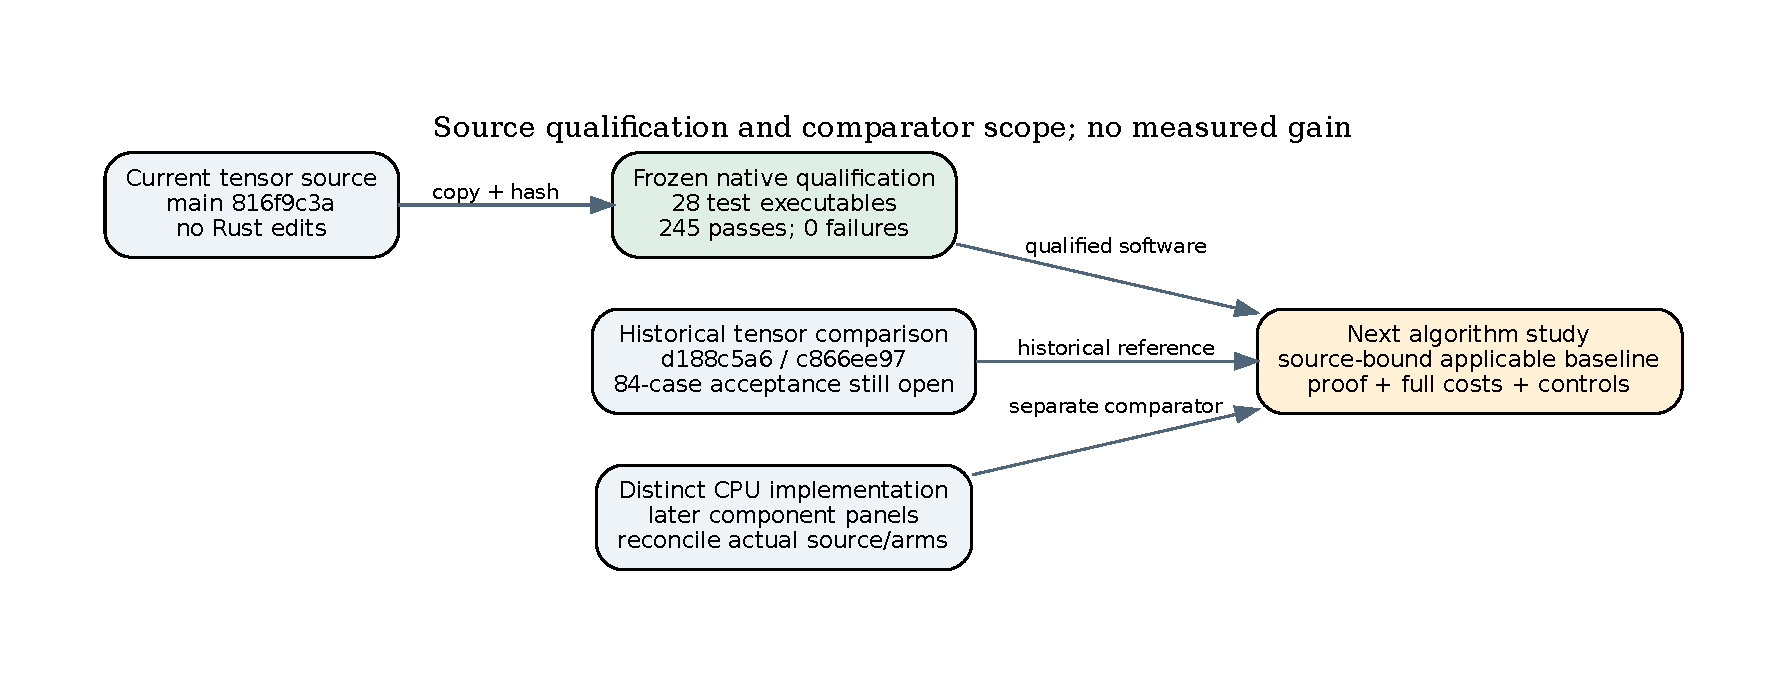
\includegraphics[width=\linewidth]{baseline-map.pdf}

Raw test times and cgroup memory readings are local development diagnostics;
they are not matched solver performance evidence. Forced recursive controls
exercise bounded arithmetic below the public admission threshold and do not
prove the external asymptotic result.

\newpage
{\Large\bfseries Comparator map and next discriminating work}

Historical records are read at producer standing under
\texttt{PCC-20261123-3d00d0}; no historical scientific execution was repeated.
Earlier comparison and later sizing binaries have distinct digests;
current option switches do not reconstruct the old source.

\begin{tabular}{@{}p{0.25\linewidth}p{0.70\linewidth}@{}}\toprule
Work & Recorded reference and remaining obligation \\\midrule
Frozen tensor panel & Baseline \texttt{d188c5a6}; sizing candidate \texttt{c866ee97}.
Only two cases with one A/A and one A/B round are recorded in that diagnostic.
The full 84-case acceptance remains open.\\
Current tensor code & Main \texttt{816f9c3a} includes later encoding reductions,
compressed coordinates and optional point-table/collector paths. Repeating
these mechanisms alone is not an untried idea.\\
CPU hashed ECDLP & Separate implementation and later component panels, including
round18 and round23. Reconcile actual arm sources and protocols before selecting
the applicable CPU comparator; historical L0 statements are not current L2 results.\\\bottomrule
\end{tabular}

\textbf{Next proof audit.} The existing November 15 dimension study leaves a
specific gap: bind inherited \texttt{child\_precision} to Appendix D.11's sharp
tapered bound, then account for attempted modes, retained vector capacities and
entry bit work. Its coarse polynomial envelope does not supply the sharper
branching exponent. Read the exact primary proof and prior tuple/packet work
before implementing another mechanism. Preserve any first exact disagreement.

\textbf{Next solver comparison.} Identify a distinct candidate, freeze its
current comparator and full cost scope, preserve all failed attempts, and
include cold setup, recovery and final replay. Field size, subgroup size,
component cost, preprocessing and number of targets must be stated before an
exponent improvement is assessed. No new candidate or exponent result is
asserted by this qualification.

\textbf{Access and failures.} KB MCP tools are unavailable and the repository
wrapper exits127 for a missing executable. Conductor is absent (exit127).
An initial sparse-helper call rejected the manually initialized sparse profile;
Git also rejected an unsupported add option. Native Git sparse-add then
materialized the same requested paths. These setup errors were retained; no
cryptographic control or theorem guard changed. KB absence prevents a novelty
clearance, not continued source work.

\textbf{Evidence.} The companion README links the frozen protocol, comparison
status, actual sizing identity, later tensor and CPU studies, raw native test
outputs and distinct build/pre-call/post-call manifests. The 66,102-byte raw
compiler JSON remains in the local capsule with its digest; its size exceeds
the repository's 64 KiB JSON-data publication threshold. S3 remains unused.
All other retained old reports and benchmark values stay unchanged.

\textbf{Review scope.} A component evidence review checks the execution record
and comparator interpretation. It is separate from a signed PCC execution
verdict or independent mathematical breakthrough review. Doctests, strict lint,
Rust 1.78 compatibility and root regression were not run here. The general counter
audit and larger complete-solver comparison remain open.

\small Repository: \url{https://github.com/isogeny-labs/crypto/pull/4996}.

Source-linked study: \path{research/hashed_ecdl_native_baseline_20261123}.
\end{document}
